\begin{surferIntroPage}{Verdensrekordflater}{record_chmutovoktic}{Flater med verdensrekord}
	En flate kalles glatt dersom den ikke har noen toppunkter (slike punkter kalles singulariteter). 
	Eksempler på glatte flater er en kule eller en torus, se de to første bildene under. 
	Velger man seg en tilfeldig flate, er den nesten alltid glatt.
 \begin{center}
      \vspace{-0.2cm}
      \begin{tabular}{@{}c@{}c@{}c@{\quad}c@{}c@{}c@{}c@{}}
        \begin{tabular}{@{}c@{}}
          Glatt:
        \end{tabular}
        &
        \begin{tabular}{@{}c@{}}
          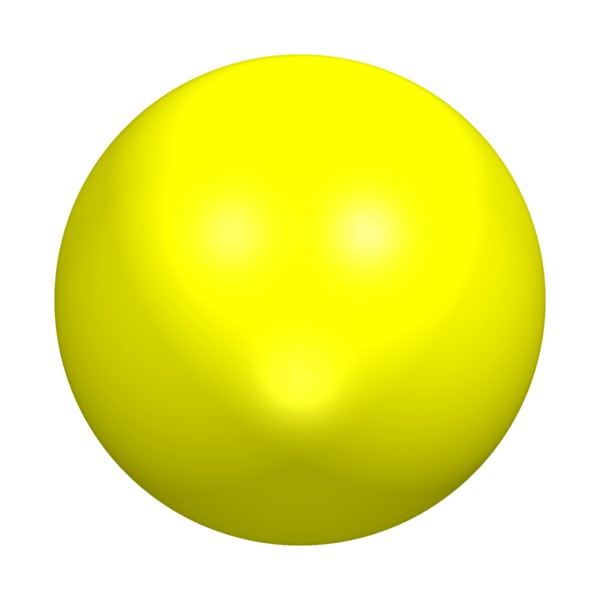
\includegraphics[width=1.1cm]{kugel}
        \end{tabular}
        &
        \begin{tabular}{@{}c@{}}
          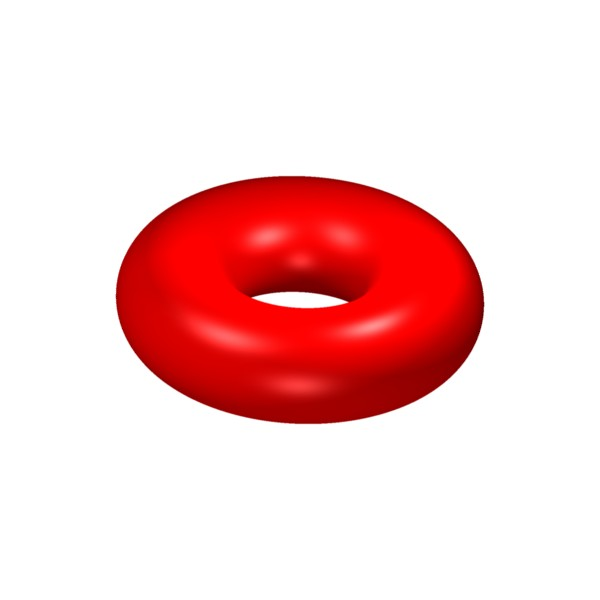
\includegraphics[width=1.1cm]{torus}
        \end{tabular}
        &
        \begin{tabular}{@{}c@{}}
          Mange\\
          singulariteter:
        \end{tabular}
        &
        \begin{tabular}{c@{}@{}}
          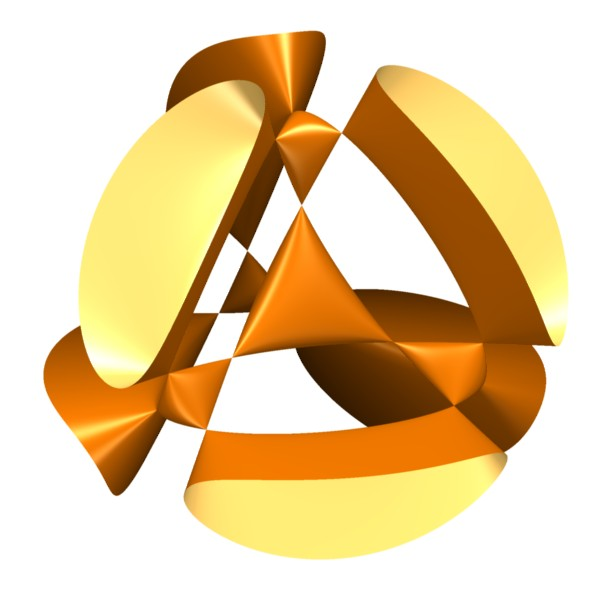
\includegraphics[width=1.1cm]{kummer}
        \end{tabular}
        &
        \begin{tabular}{c@{}@{}}
          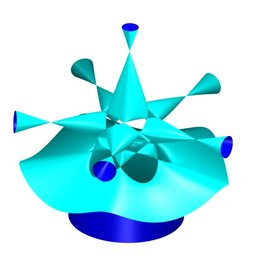
\includegraphics[width=1.1cm]{togliatti}
        \end{tabular}
        &
        \begin{tabular}{c@{}@{}}
          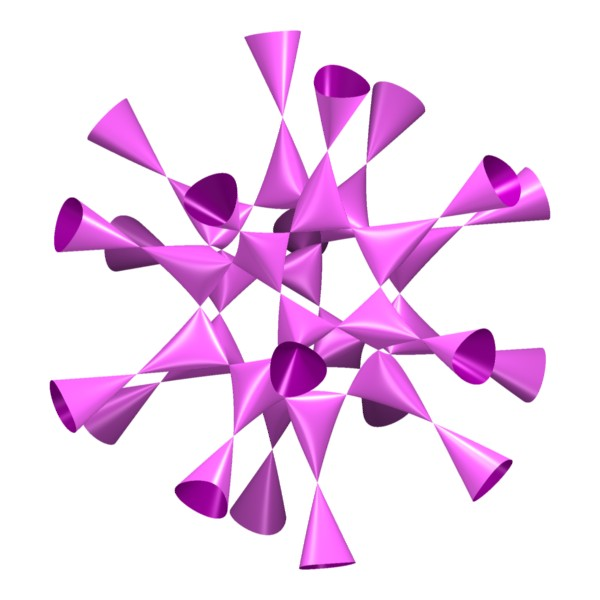
\includegraphics[width=1.1cm]{barth_sextic}
        \end{tabular}
      \end{tabular}
    \end{center}
    \vspace{-0.2cm}
	
	Bare spesielle flater har singulariteter. Det gjør singularitetene til flatenes mest 
  interessante punkter. Flatene i programmet SURFER er definert av polynomer. Den høyeste 
  eksponenten til et polynom kalles graden til polynomet. Matematikere spør seg hvor mange
  singulariteter en flate av en bestemt grad kan ha. Vi kaller dette antallet for $\mu(d)$. 
  
  Det viser seg at antallet $\mu(d)$ er veldig vanskelig å beregne. Siden 1800-tallet har $\mu(d)$ 
  vært kjent for $d=1,2,3,4$, men ikke før i 1980 fant man det for $d=5$, og i 1996 for $d=6$.
  For $d\ge 7$, $\mu(d)$ fortsatt ukjent. 

  Enhver ny verdensrekord for $\mu(d)$ er derfor viktig. Det ser ut til å ta tid å finne en komplett løsning av $\mu(d)$ for en 
  vilkårlig $d$.\\ Her følger noen kjente resultater:
  
    
   \begin{center}
      \begin{tabular}{r|cccccccc|c}
        $d$ & $1$ & $2$ & $3$ & $4$ & $5$ & $6$ & $7$ & $8$ & $d$\\
        \hline
        \hline
        \rule{0pt}{1.2em}$\mu(d)\ge$ & $0$ & $1$ & $4$ & $16$ & $31$ & $65$ &
        $99$ & $168$ & 
        $\approx \frac{5}{12}d^3$\\[0.3em]
        \hline
        \rule{0pt}{1.2em}$\mu(d)\le$ & $0$ & $1$ & $4$ & $16$ & $31$ & $65$ &
        $104$ & $174$ & $\approx \frac{4}{9}d^3$
      \end{tabular}
    \end{center}
\end{surferIntroPage}
